\documentclass[12pt,letterpaper,titlepage]{article}
\usepackage[margin=1in]{geometry}
\usepackage{minted}
\usepackage{float, graphicx}
\usepackage{hyperref}
\setminted{autogobble, mathescape}
\usemintedstyle{tango}

\title{CSCI 403 Final Project:\\
       A Better Mines Courses Database}
\date{\today}
\author{Jack Rosenthal, Ariel Shlosberg, Nicholas Lantz\\
        \small CSCI 403\\
        \small Dr. Christopher Painter-Wakefield\\
        \small Colorado School of Mines}

\begin{document}
\maketitle

\section{The Data Set}
The data set that was used for this project was course information obtained by parsing the HTML on banner.mines.edu. This is very similar to the course information that was presented to us in CPW's database, however we gain the advantage of being able to select the course information from any available previous term or even next semester's course information. This is an interesting data set as it allows us to look for historical trends in Mines courses over the years as well as to try to find interesting correlations and statistics about the classes next semester. The data is initially very flat as presented in banner and separates each course section into a separate object. This means that the first step of working with the data and importing it into the database was to determine the best way to represent the data set in a normalized format. We decided to break our data into four separate tables representing the different major components in describing a course (instructor, course, section, and meeting). This allowed us to effectively normalize the database using BCNF as was shown in class. Each table has corresponding attributes that are necessary to describing the entity, but the overall structure is such that data redundancy is minimized and data integrity is preserved. An example of each of the relations is presented below in Figure \ref{tbl:instructor} through Figure \ref{tbl:course}.

\begin{table}[H]
\centering
\begin{tabular}{|c|c|}
\hline
meeting\_id & name \\ \hline
22 & C Joshua Ramey \\ \hline
23 & Judith Nickolls Schoonmaker \\ \hline
24 & Judith Nickolls Schoonmaker \\ \hline
25 & Paul Carr Johnson \\ \hline
26 & Tracy Q. Gardner \\ \hline
27 & Tracy Q. Gardner \\ \hline
28 & Jason C Ganley \\ \hline
29 & Jason C Ganley \\ \hline
\end{tabular}
\caption{\label{tbl:instructor} Example of instructor relation}
\end{table}

\begin{table}[H]
\footnotesize
\centering
\begin{tabular}{|c|c|c|c|c|c|c|c|c|}
\hline
id & crn & begin\_time & end\_time & days & begin\_date & end\_date & loc\_building & loc\_room \\ \hline
22 & 12685 & 08:00 & 09:50 & MWF & 2017-01-10 & 2017-05-12 & Alderson Hall & 291 \\ \hline
23 & 12686 & 10:00 & 11:50 & MWF & 2017-01-10 & 2017-05-12 & Alderson Hall & 291 \\ \hline
24 & 12687 & 14:00 & 16:45 & TR & 2017-01-10 & 2017-05-12 & Alderson Hall & 291 \\ \hline
25 & 12314 & 07:30 & 08:45 & MW & 2017-01-10 & 2017-05-12 & Alderson Hall & 230 \\ \hline
26 & 12316 & 09:00 & 09:50 & MWF & 2017-01-10 & 2017-05-12 & Alderson Hall & 230 \\ \hline
27 & 11084 & 11:00 & 11:50 & MWF & 2017-01-10 & 2017-05-12 & Brown Building & W250 \\ \hline
28 & 11085 & 08:00 & 09:15 & T & 2017-01-10 & 2017-05-12 & Alderson Hall & 162 \\ \hline
29 & 11086 & 09:30 & 10:45 & T & 2017-01-10 & 2017-05-12 & Alderson Hall & 162 \\ \hline
\end{tabular}
\caption{\label{tbl:meeting} Example of meeting relation}
\end{table}

\begin{table}[H]
\centering
\begin{tabular}{|c|c|c|c|c|}
\hline
crn & course\_id & section\_letter & min\_credits & max\_credits \\ \hline
10622 & 9 & A & 0.000 & 0.000 \\ \hline
12685 & 10 & A & 4.000 & 4.000 \\ \hline
12686 & 10 & B & 4.000 & 4.000 \\ \hline
12687 & 11 & A & 4.000 & 4.000 \\ \hline
12314 & 12 & A & 3.000 & 3.000 \\ \hline
12316 & 12 & B & 3.000 & 3.000 \\ \hline
11084 & 12 & C & 3.000 & 3.000 \\ \hline
11085 & 13 & A & 1.000 & 1.000 \\ \hline
\end{tabular}
\caption{\label{tbl:section} Example of section relation}
\end{table}

\begin{table}[H]
\centering
\begin{tabular}{|c|c|c|c|}
\hline
id & title & subject & number \\ \hline
8 & ENGINEERING YOUR CAREER PATH & CSM & 250 \\ \hline
9 & INTERNATIONAL THESIS CPT & CSM & 597A \\ \hline
10 & FUNDAMENTALS OF BIOLOGY I & CBEN & 110 \\ \hline
11 & FUNDAMENTALS OF BIOLOGY II & CBEN & 120 \\ \hline
12 & MATERIAL AND ENERGY BALANCES & CBEN & 201 \\ \hline
13 & CHEMICAL PROCESS PRINCIPLES LABORATORY & CBEN & 202 \\ \hline
14 & INTRO TO THERMODYNAMICS & CBEN & 210 \\ \hline
15 & HEAT TRANSFER & CBEN & 308 \\ \hline
\end{tabular}
\caption{\label{tbl:course}Example of course relation}
\end{table}

The instructor relation, as seen in Table \ref{tbl:instructor}, is quite simple and is only composed of the instructor's name and one of the meeting\_id's associated with the meeting that the instructor teaches. Combined they serve as a primary key for the instructor table (e.g. (22, Joshua Ramsey) serves as a primary key in Table \ref{tbl:instructor}). The instructor table is essentially a cross-reference table since the instructor meeting relationship is a many-to-many relationship (N to M). This is because a single instructor can instruct many meetings and a single meeting can have multiple instructors. The meeting relation, as seen in Table \ref{tbl:meeting}, stores all of the meeting specific information such as the crn associated with a certain section (foreign key constraint back to the section relation), the course's meeting location, days, times, and the dates through which the course runs. Each tuple in the meeting relation has an associated id that serves as the primary key for the relation. There are no other foreign dependencies in the meeting relation. The section relation, shown in Table \ref{tbl:section}, essentially just lists out all of the different sections associated with a certain course (using a foreign key on the course\_id attribute back to the course relation), the credit range associated with the section, and the crn of the section that acts as the primary key for the relation. Each crn is unique for a section as opposed to for a course, but a single crn can still have multiple different meeting times and locations. Finally, the course relation, shown in Table \ref{tbl:course}, gives the course id (which serves as the primary key), the course title, and the subject id and number.

% Interesting things about dataset, where it was obtained, licensing (lol)
% Description of tables
\section{Cool Things}
After setting up the relations on CPW's database it was possible to perform some interesting queries on the data. The first thing that was investigated was the course distribution as a function of start time throughout the day shown in Figure \ref{fig:starthours}.

\begin{figure}[H]
\centering
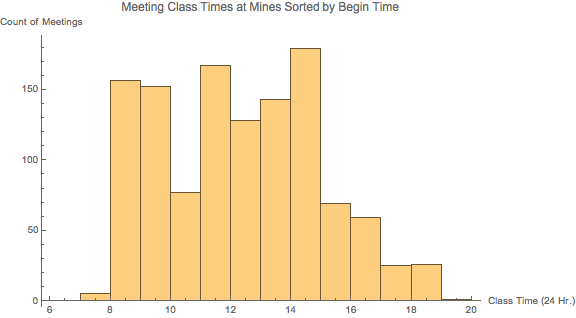
\includegraphics[width = 4 in]{classmeetinghist.png}
\caption{\label{fig:starthours}Plot of the number of course meetings on campus as function start time}
\end{figure}

The distribution of class times does not appear very Gaussian as might be expected, however there are clearly more meeting times from 8-3 than in the very early morning or late in the afternoon. The most popular time of day to take a class is at 2 and there also appears to be a somewhat strange drop in meeting times from 10-11. 

% Need ideas for this section, currently have...
% Explosion of Computer Science Popularity

\section{Technical Challenges}

The largest challenge associated with this project was parsing the data from
the \emph{Self Service Banner} (SSB) system. The \emph{Dynamic Schedule} page
on SSB provides a very flat listing of all sections without authentication to
the Mines system, which allows for easy importing. The URL to access this page
is at:

\begin{center}
    \url{https://banner.mines.edu/prod/owa/bwckschd.p_disp_dyn_sched}
\end{center}

Parsing through this was a hot mess. Looking at the HTML output from SSB, it's
surprising that most web browsers are even capable of properly rendering the
page. Some of the nasties included nested HTML tables without proper closing
tags.

\begin{figure}[H]
    \centering
    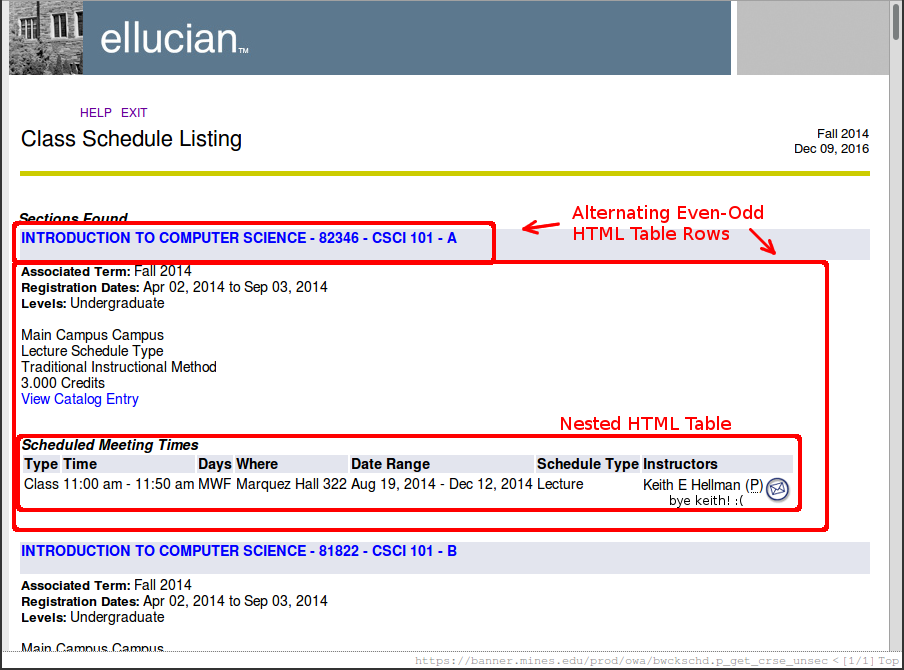
\includegraphics[width=0.8\linewidth]{bannertbl.png}
    \caption{Screenshot depicting the HTML structure of the page parsed}
\end{figure}

Fortunately, the \emph{Beautiful Soup 4} library for Python (in combination
with \emph{lxml}) was able to help remove inconsistencies, like the lack of a
proper XML structure. Through this, our data could be obtained using a simple
pairwise iteration of the outermost even-odd HTML table rows and a few PCREs.



\end{document}
